% FHOPS manuscript (SoftwareX submission wrapper)
\documentclass[preprint,review,12pt]{elsarticle}

\usepackage{hyperref}
\pdfstringdefDisableCommands{%
  \def\corref#1{}%
  \def\cortext#1#2{}%
  \def\ead#1{}%
}
\usepackage{amsmath}
\usepackage{amssymb}
\usepackage{textcomp}
\usepackage{lineno}
\usepackage{tikz}
\usetikzlibrary{positioning,arrows.meta}
\usepackage{booktabs}
\usepackage{longtable}
\usepackage{array}
\usepackage{calc}
\modulolinenumbers[5]

\providecommand{\tightlist}{%
  \setlength{\itemsep}{0pt}\setlength{\parskip}{0pt}}
\newcommand{\breakpath}[1]{\path{#1}}

\journal{SoftwareX}

% Shared metadata macros will live here later

\begin{document}

\begin{frontmatter}

\title{FHOPS: a reproducible optimisation and benchmarking stack for forest harvest operations}

\author[ubc]{Gregory Paradis\corref{cor1}}
\ead{gregory.paradis@ubc.ca}
\author[ubc]{Rosalia Jaffray}
\author[ubc]{Kathleen Coupland}
\cortext[cor1]{Corresponding author. Tel.: +1 604 822 1890.}
\address[ubc]{Faculty of Forestry, University of British Columbia, 2424 Main Mall,
Office 4645, Vancouver, British Columbia, V6T 1Z4, Canada}

% Highlights placeholder
\section*{Highlights}
\begin{itemize}
  \item FHOPS standardizes harvest planning inputs for comparable optimization studies.
  \item Heuristic and MILP solvers share one auditable formulation and data contract.
  \item Benchmark, playback, and costing outputs are reproducible from versioned assets.
\end{itemize}


\begin{abstract}
Operational forest machine scheduling remains dominated by site-specific tools that are difficult to transfer, audit, and compare across studies. The recent systematic review by Jaffray et~al. highlights this gap and calls for reusable, transparent planning workflows. FHOPS addresses that requirement by providing an open-source operational planning platform built around a common scenario contract, a solver stack (mixed-integer programming plus SA/ILS/Tabu heuristics), and a unified evaluation layer for schedule quality, robustness, and cost interpretation. We demonstrate the platform on a reproducible British Columbia ground-based dataset ladder (tiny7, small21, med42) plus synthetic scaling tiers, with manuscript tables and figures generated directly from versioned benchmark assets. This paper therefore documents the reusable software platform and baseline evidence; detailed rolling-horizon design analysis and broader deployment studies are treated as companion modelling work.
\end{abstract}


\begin{keyword}
forest operations \sep optimisation \sep reproducibility \sep heuristics \sep Pyomo \sep telemetry
\end{keyword}

% Code metadata table (journal requirement)
\begin{table}[ht]
  \centering
  \caption{Code metadata (reproducibility requirement)}
  \label{tab:code-metadata}
  \begin{tabular}{p{0.35\linewidth}p{0.55\linewidth}}
    \hline
    Current code version & FHOPS 1.0.0 (GitHub tag \texttt{v1.0.0}) \\
    Permanent link to code/repository & \url{https://github.com/UBC-FRESH/fhops/tree/v1.0.0} \\
    Legal Code License & MIT License (OSI approved) \\
    Computing platforms/requirements & GNU/Linux (Ubuntu 24.04 LTS CI target), macOS, Windows via WSL2; Python 3.11 or newer; optional CUDA GPU for stochastic playback batches \\
    Installation requirements & Install the published package with \texttt{pip install fhops==1.0.0}, or check out tag \texttt{v1.0.0} and use the Hatch-managed development workflow (\texttt{hatch run dev:suite}). HiGHS binaries are vendored via PyPI wheels. \\
    Documentation link & \url{https://ubc-fresh.github.io/fhops/} \\
    Reproducibility log & \texttt{docs/softwarex/assets/benchmark\_runs.log} records every \texttt{make manuscript-benchmarks} run (commit, runtime, SHA-256 hash); artefacts live under \texttt{docs/softwarex/assets/**}. \\
    Support contact & gregory.paradis@ubc.ca (Faculty of Forestry, UBC) \\
    \hline
  \end{tabular}
\end{table}

% Current code version table (journal requirement)
\begin{table}[ht]
  \centering
  \caption{Current code version details}
  \label{tab:current-code-version}
  \scriptsize
  \begin{tabular}{>{\raggedright\arraybackslash}p{0.30\linewidth}>{\raggedright\arraybackslash}p{0.60\linewidth}}
    \hline
    Software version & FHOPS 1.0.0 (GitHub tag \texttt{v1.0.0}) \\
    Permanent link to executables/code & GitHub release: \url{https://github.com/UBC-FRESH/fhops/releases/tag/v1.0.0}; PyPI package: \url{https://pypi.org/project/fhops/1.0.0/} \\
    Operating systems & Ubuntu 24.04 LTS (CI default), macOS, Windows via WSL2 \\
    Dependencies & Python 3.11+, Pyomo 6.7+, HiGHS 1.7+ via \texttt{highspy}, NumPy 1.26+, Pandas 2.2+, Optuna 3.5+; optional Gurobi 11.0+ \\
    Installation method & Install with \texttt{pip install fhops==1.0.0}, or use the Hatch development environment (\texttt{hatch run dev:suite}) \\
    Build system & Hatch (PEP~517 backend defined in \texttt{pyproject.toml}) \\
    Continuous integration & GitHub Actions (linux/macos/windows) badge: \url{https://github.com/UBC-FRESH/fhops/actions} \\
    Reproducibility evidence & \texttt{make manuscript-benchmarks} regenerates all assets and logs hashes to \breakpath{docs/softwarex/assets/benchmark_runs.log} \\
    \hline
  \end{tabular}
\end{table}


\end{frontmatter}

\linenumbers

% Section 1: Motivation and significance
\section{Motivation and significance}
\label{sec:introduction}

Forest operations planners make short-horizon decisions about machine allocation,
sequence, and timing under binding logistical constraints. These decisions are evaluated against cost, safety, environmental performance, and reliability of delivery, while operating conditions vary between tenure, terrain, and harvest systems
\cite{henkelman1978gpssv,weintraub1996new,heinimann2007forest};
decision-support systems have long treated these settings as optimization problems
\cite{buongiorno2003decision,kangas2008decision}.
In practice, organizations still combine spreadsheets, geographic information system (GIS) workflows, and local scripts for day-to-day scheduling,  limiting comparability and slowing model transfer
\cite{ulvdal2022uncertainty,nelson2003forestmodels}.

The systematic review by Jaffray et al.~provides the clearest current synthesis of this problem space \cite{jaffray2025systematic}. Among 23 peer-reviewed studies published between 2005 and 2024, the review reports strong technical contributions but recurring structural limitations: high site specificity, limited open artifacts, and weak or no reproducibility support. The design implications of the review are explicit: operational planning tools need standardized inputs, transparent formulations, and reproducible evaluation workflows. These changes in operational planning tools will allow methods, identification of recurring limiting factors and spatial impacts to be compared without rebuilding full software stacks.

This SoftwareX paper is the middle contribution in a review $\rightarrow$ platform $\rightarrow$ modelling sequence. The review defines the gap and requirements; this paper documents the Forest Harvesting Operations Planning System (FHOPS) as reusable infrastructure that operationalizes those requirements and produces a reproducible baseline evidence package; follow-up modelling work then deploys FHOPS on a number of case studies to explore specific design questions (e.g., rolling-horizon configuration) on that shared baseline.

FHOPS combines a scenario contract for operational inputs, heuristic and mixed-integer exact solver pathways, and a shared evaluation layer for runtime, schedule quality, robustness, and costing interpretation. In this context, FHOPS executes machine scheduling in forest operations as a structured, scenario-driven optimization problem with explicit resource, sequencing and timing decisions. The contribution is not a new optimization theorem; it is a reusable, inspectable software that enables equivalent experiments on shared structures with traceable outputs.

In this paper, we make three contributions.
\begin{enumerate}
  \item \textbf{Operational planning software architecture.} We define a domain-first software structure around blocks, machines, shifts, landings, and mobilization rules allowing scheduling analyses that are transferrable across cases with minimal recoding.
  \item \textbf{Canonical formulation + traceability.} We present the operational mixed-integer linear program (MILP) in a canonical equation block with direct links to implementation and regression tests, enabling reviewer-level verification from manuscript equation to executable model.
  \item \textbf{Reproducible validation baseline.} We report benchmark, tuning, playback-robustness, and costing outputs on a public British Columbia (BC) reference ladder (tiny7, small21, med42), with synthetic scaling support, so future modelling studies can reuse a stable baseline.
\end{enumerate}

Scope is intentionally bounded. We focus on software platform capability and reproducible baseline evidence, not on broad claims of external deployment impact. Real-world multi-context validation (including additional system families and rolling-horizon case analyses) is treated as downstream modelling work that reuses the same platform and artifacts rather than redefining them.

Section~\ref{sec:software-description} describes entities, methods, and formulation traceability. Section~\ref{sec:illustrative-example} reports validation evidence around planner-facing operational questions. Section~\ref{sec:impact} discusses deployment relevance, maturity, and transfer limits. Section~\ref{sec:conclusions} closes with claims, limits, and the handoff to companion modelling studies.

% Section 2: Software description
\section{Software description}
\label{sec:software-description}

FHOPS is organized around the core operational scheduling question: given a set of blocks, machine resources, shift calendars, and mobilization constraints, what assignments should be made, in which sequence, and with what expected production and cost consequences. The software architecture is therefore defined by planning entities and decision logic first, and by implementation boundaries second.

\subsection{Operational entities and planning context}
The platform uses a typed scenario contract allowing solver results to be compared on fixed operational inputs:
\begin{itemize}
  \item \textbf{Blocks and windows}: harvest volumes, treatment windows, and system requirements.
  \item \textbf{Machines and roles}: role-specific production rates, availability, and compatibility.
  \item \textbf{Shift calendar}: day-shift time grid used for assignment and production accounting.
  \item \textbf{Landings and mobilization}: movement penalties and daily landing capacities.
  \item \textbf{Constraint metadata}: sequencing prerequisites, role activation conditions, and completion balances.
\end{itemize}

FHOPS ships a public BC ground-based reference ladder (tiny7, small21, med42) that scales from 7/2 to 21/6 to 42/12 (days/blocks) while keeping one operational archetype.

This addresses a central review finding \cite{jaffray2025systematic}: transfer fails when assumptions are embedded in bespoke code rather than explicit scenario data. Generalizability is supported structurally through this scenario contract, which separates operational assumptions from solver logic. Empirical validation across additional system families remains future work.

\subsection{Solution methods for operational decisions}
FHOPS provides complementary solver families for different planning horizons and time budgets:
\begin{itemize}
  \item \textbf{Metaheuristic solvers (SA/ILS/Tabu)} provide practical schedule candidates for larger instances where rapid re-solving is needed.
  \item \textbf{Mixed-integer linear programming (MILP)} provides an exact baseline where tractable, supporting verification and sensitivity analysis.
  \item \textbf{Playback evaluation} re-simulates solved schedules under deterministic and stochastic conditions to quantify utilization, continuity, and disruption effects.
\end{itemize}

This reflects established forestry operations research (OR) practice: exact models support formulation clarity and benchmark bounds, while heuristics support larger-scale operational runs \cite{paradis2018bilevel,nelson2003forestmodels}.

Warm-start support is implemented for MIP, but this paper does not claim decisive wall-clock gains on med42/large84 stress contexts.

\subsection{Operational MILP and equation-to-code traceability}
The deterministic operational MILP is presented in canonical form below. Equation blocks are labeled as OBJ, E1--E11, and D1.

% AUTO-GENERATED from fhops_operational_formulation.md -- do not edit directly.
FHOPS' deterministic operational solver is defined on a day-shift grid.
It maximizes delivered production and penalizes unmet volume,
landing-capacity surplus, and machine transitions. Equation blocks below
are the canonical manuscript/docs reference and map directly to
implementation.

\textbf{Problem statement.} Given blocks, machine roles, calendars,
windows, and landing capacities, choose machine-block assignments and
per-shift production to maximize weighted output under feasibility and
sequencing constraints.

\textbf{Sets and indices.}

\begin{itemize}
\tightlist
\item
  \(m \in \mathcal{M}\): machines.
\item
  \(b \in \mathcal{B}\): blocks.
\item
  \(s=(d,\sigma) \in \mathcal{S}\): shift slots (day \(d\), shift label
  \(\sigma\)).
\item
  \(\mathcal{R}_b\): ordered roles required on block \(b\).
\item
  \(\mathcal{L}\): landings.
\item
  \(\mathcal{P}^{\text{inv}}\): role-block pairs with upstream
  prerequisites.
\item
  \(\mathcal{P}^{\text{act}} \subseteq \mathcal{P}^{\text{inv}}\):
  role-block pairs requiring head-start activation.
\item
  \(\mathcal{P}^{\text{load}}\): loader role-block pairs.
\end{itemize}

\textbf{Parameters.}

\begin{itemize}
\tightlist
\item
  \(\bar{p}_{mb}\): production rate for machine \(m\) on block \(b\).
\item
  \(W_b\): required total block production volume.
\item
  \(A_{m,s} \in \{0,1\}\): machine availability for shift \(s\).
\item
  \(\mathbf{1}^{\text{window}}_{b,d} \in \{0,1\}\): block window
  indicator.
\item
  \(\omega^{\text{prod}},\omega^{\text{mob}},\omega^{\text{trans}},\omega^{\text{land}}\):
  objective weights.
\item
  \(\delta_{m,b',b}\): mobilization cost when machine \(m\) transitions
  from block \(b'\) to block \(b\).
\item
  \(C_{\ell}\): daily assignment capacity for landing \(\ell\).
\item
  \(\ell(b)\): landing associated with block \(b\).
\item
  \(\mathcal{U}_{r,b}\): upstream roles that must feed role \(r\) on
  block \(b\).
\item
  \(B_{r,b}\): required staged buffer volume before role \(r\) may
  activate on block \(b\).
\item
  \(Q_{r,b}\): role production capacity upper bound per shift (used for
  activation linearization).
\item
  \(q^{\text{batch}}_{r,b}\): loader batch size for loader role \(r\) on
  block \(b\).
\item
  \(\mathcal{T}_b \subseteq \mathcal{R}_b\): terminal roles for block
  \(b\).
\end{itemize}

\textbf{Decision variables.}

\begin{itemize}
\tightlist
\item
  \(x_{m,b,s} \in \{0,1\}\): 1 if machine \(m\) is assigned to block
  \(b\) in shift \(s\).
\item
  \(p_{m,b,s} \ge 0\): production by machine \(m\) on block \(b\) in
  shift \(s\).
\item
  \(z_{r,b,s} \ge 0\): aggregated role-level production for role \(r\)
  on block \(b\) in shift \(s\).
\item
  \(y_{m,b',b,s} \in \{0,1\}\): transition indicator from previous-shift
  block \(b'\) to current block \(b\) (non-initial shifts).
\item
  \(I^{\text{start}}_{r,b,s} \ge 0\): staged inventory available at
  start of shift \(s\) for role \(r\) on block \(b\).
\item
  \(I_{r,b,s} \ge 0\): staged inventory at end of shift \(s\) for role
  \(r\) on block \(b\).
\item
  \(g_{r,b,s} \in \{0,1\}\): role activation indicator for buffered
  downstream roles.
\item
  \(n_{r,b,s} \in \mathbb{Z}_{\ge 0}\): loader batch count for loader
  role-block pair \((r,b)\).
\item
  \(u_{r,b,s} \ge 0\): loader partial remainder volume.
\item
  \(L_b \ge 0\): leftover unmet block volume slack.
\item
  \(S_{\ell,d} \ge 0\): landing daily surplus slack.
\end{itemize}

\textbf{Objective.}

FHOPS maximizes weighted terminal production and subtracts penalty
terms:

\[
\begin{aligned}
\max\; &\omega^{\text{prod}}\!\sum_{b\in\mathcal{B}}\sum_{r\in\mathcal{T}_b}\sum_{s\in\mathcal{S}} z_{r,b,s}
- \omega^{\text{prod}}\!\sum_{b\in\mathcal{B}} L_b \\
&- \omega^{\text{land}}\!\sum_{\ell\in\mathcal{L}}\sum_{d\in\mathcal{D}} S_{\ell,d} \\
&- \omega^{\text{mob}}\!\sum_{m,b',b,s} \delta_{m,b',b}\, y_{m,b',b,s}
- \omega^{\text{trans}}\!\sum_{m,b',b,s} y_{m,b',b,s}.
\end{aligned}
\]

If a block has no terminal-role metadata, implementation falls back to
machine-level production sums for the production-reward term.

\textbf{Constraints.} For traceability, the objective is tagged as
\textbf{OBJ}, constraints as \textbf{E1--E11}, and domain declarations
as \textbf{D1}.

Machine assignment feasibility (\textbf{E1}):

\[
\sum_{b\in\mathcal{B}} x_{m,b,s} \le A_{m,s}
\qquad \forall m\in\mathcal{M},\; s\in\mathcal{S}.
\]

Role compatibility (\textbf{E2}, machines can only work roles allowed by
the block's assigned harvest system):

\[
x_{m,b,s}=0 \quad \text{if role}(m)\notin\mathcal{R}_b.
\]

Production upper bound per assignment (\textbf{E3}):

\[
p_{m,b,s} \le \bar{p}_{mb}\,x_{m,b,s}
\qquad \forall m,b,s.
\]

Block window enforcement (\textbf{E4}):

\[
x_{m,b,s}=0 \quad \text{if } \mathbf{1}^{\text{window}}_{b,d}=0 \text{ for } s=(d,\sigma).
\]

Role-production aggregation (\textbf{E5}):

\[
z_{r,b,s} = \sum_{m\in\mathcal{M}(r)} p_{m,b,s}
\qquad \forall (r,b), s.
\]

Transition linking (\textbf{E6}, for non-initial shifts only):

\[
y_{m,b',b,s} \le x_{m,b',\operatorname{prev}(s)},
\qquad
y_{m,b',b,s} \le x_{m,b,s},
\] \[
y_{m,b',b,s} \ge x_{m,b',\operatorname{prev}(s)} + x_{m,b,s} - 1.
\]

Role inventory start and balance for prerequisite-driven downstream
roles (\textbf{E7}):

\[
I^{\text{start}}_{r,b,s}=
\begin{cases}
0, & s \text{ is first shift}\\
I_{r,b,\operatorname{prev}(s)}, & \text{otherwise}
\end{cases}
\qquad \forall (r,b)\in\mathcal{P}^{\text{inv}}, s,
\]

\[
I_{r,b,s}=I^{\text{start}}_{r,b,s}+\sum_{u\in\mathcal{U}_{r,b}} z_{u,b,s}-z_{r,b,s}
\qquad \forall (r,b)\in\mathcal{P}^{\text{inv}}, s,
\]

\[
z_{r,b,s} \le I^{\text{start}}_{r,b,s}
\qquad \forall (r,b)\in\mathcal{P}^{\text{inv}}, s.
\]

Head-start activation for buffered downstream roles (\textbf{E8}):

\[
z_{r,b,s} \le Q_{r,b}\,g_{r,b,s}
\qquad \forall (r,b)\in\mathcal{P}^{\text{act}}, s,
\]

\[
I_{r,b,\operatorname{prev}(s)} \ge B_{r,b}\,g_{r,b,s}
\qquad \forall (r,b)\in\mathcal{P}^{\text{act}}, s,
\]

\[
\sum_{m\in\mathcal{M}(r)} x_{m,b,s} \le |\mathcal{M}(r)|\, g_{r,b,s},
\qquad
g_{r,b,s} \le \sum_{m\in\mathcal{M}(r)} x_{m,b,s}
\qquad \forall (r,b)\in\mathcal{P}^{\text{act}}, s.
\]

Loader batching (\textbf{E9}):

\[
z_{r,b,s}=q^{\text{batch}}_{r,b}\,n_{r,b,s}+u_{r,b,s}
\qquad \forall (r,b)\in\mathcal{P}^{\text{load}}, s,
\]

\[
0 \le u_{r,b,s} \le q^{\text{batch}}_{r,b}
\qquad \forall (r,b)\in\mathcal{P}^{\text{load}}, s.
\]

Block completion balance with leftover slack (\textbf{E10}):

\[
\sum_{r\in\mathcal{T}_b}\sum_{s\in\mathcal{S}} z_{r,b,s} + L_b = W_b
\qquad \forall b\in\mathcal{B}.
\]

Landing daily assignment capacity with surplus slack (\textbf{E11}):

\[
\sum_{b:\,\ell(b)=\ell}\sum_{m\in\mathcal{M}}\sum_{\sigma:(d,\sigma)\in\mathcal{S}} x_{m,b,(d,\sigma)}
\le C_{\ell} + S_{\ell,d}
\qquad \forall \ell\in\mathcal{L},\; d\in\mathcal{D}.
\]

Domain restrictions (\textbf{D1}):

\[
x, y, g \in \{0,1\},\quad n \in \mathbb{Z}_{\ge 0},\quad p,z,I^{\text{start}},I,u,L,S \ge 0.
\]

\textbf{Implementation mapping (equation blocks to code).}

Primary modules: \texttt{src/fhops/model/milp/operational.py},
\texttt{src/fhops/model/milp/data.py}. Primary tests:
\texttt{tests/model/test\_operational\_milp.py},
\texttt{tests/model/test\_operational\_driver.py}.

Equation-block mapping:

\begin{itemize}
\tightlist
\item
  \textbf{OBJ}: \texttt{model.objective} with \texttt{prod\_weight},
  \texttt{landing\_weight}, \texttt{mobilisation\_weight},
  \texttt{transition\_weight}
\item
  \textbf{E1}: \texttt{model.machine\_capacity}
  (\texttt{machine\_capacity\_rule})
\item
  \textbf{E2}: \texttt{model.role\_compatibility}
  (\texttt{role\_compatibility\_rule})
\item
  \textbf{E3}: \texttt{model.production\_cap} (\texttt{prod\_cap\_rule})
\item
  \textbf{E4}: \texttt{model.block\_windows} (\texttt{window\_rule})
\item
  \textbf{E5}: \texttt{model.role\_prod\_balance}
  (\texttt{role\_prod\_balance\_rule})
\item
  \textbf{E6}: \texttt{model.transition\_prev},
  \texttt{model.transition\_curr}, \texttt{model.transition\_link}
\item
  \textbf{E7}: \texttt{model.inventory\_start\_eq},
  \texttt{model.inventory\_balance}, \texttt{model.inventory\_guard}
\item
  \textbf{E8}: \texttt{model.activation\_prod},
  \texttt{model.head\_start}, \texttt{model.role\_active\_upper},
  \texttt{model.role\_active\_lower}
\item
  \textbf{E9}: \texttt{model.loader\_batch},
  \texttt{model.loader\_partial\_cap}
\item
  \textbf{E10}: \texttt{model.block\_balance}
  (\texttt{block\_balance\_rule}) + \texttt{model.leftover}
\item
  \textbf{E11}: \texttt{model.landing\_capacity}
  (\texttt{landing\_capacity\_rule}) + \texttt{model.landing\_surplus}
\item
  \textbf{D1}: variable domain declarations for \texttt{model.x},
  \texttt{model.y}, \texttt{model.role\_active}, \texttt{model.loads},
  \texttt{model.prod}, \texttt{model.role\_prod},
  \texttt{model.inventory\_start}, \texttt{model.inventory},
  \texttt{model.loader\_partial}, \texttt{model.leftover}, and
  \texttt{model.landing\_surplus}
\end{itemize}

This formulation is the canonical mathematical reference for FHOPS
operational MILP documentation and companion modelling manuscripts.


Each block maps to named implementation objects and regression tests. The shared formulation source keeps the manuscript and documentation synchronized for auditability.
For practical review, the path is explicit: equation labels map to Pyomo objects in the operational builder, then to tests that check sequencing logic, bundle normalization, and driver integration. This design and structure reduces ambiguity when readers compare mathematical intent with executable behaviour and helps maintainers detect formulation drift when model code evolves.

\subsection{Architecture and implementation boundaries}
Internally, FHOPS separates four concerns:
\begin{enumerate}
  \item \textbf{Scenario layer}: ingestion and validation of planning entities.
  \item \textbf{Optimization layer}: heuristic and MILP solvers sharing common scenario inputs.
  \item \textbf{Evaluation layer}: playback and key performance indicators (KPI) computation for solved schedules.
  \item \textbf{Reporting layer}: generation of tables/figures used in manuscript and documentation outputs.
\end{enumerate}

The software is available through Python modules and command-line wrappers. Interface choice is secondary to preserving equivalent, traceable evidence across runs. FHOPS is released under an MIT license, with source code, datasets, and experiment pipelines in a public repository to support reuse and independent verification.

\subsection{Reproducible evidence pipeline}
Manuscript evidence comes from versioned benchmark, tuning, playback, costing, and scaling assets produced by the same platform layers. Run logs and artifact paths provide provenance for each reported value.

This arrangement is deliberate in the manuscript sequence: the review identifies missing reproducibility infrastructure \cite{jaffray2025systematic}, this paper contributes it as reusable software, and companion modelling studies can focus on method questions without redefining data contracts or reporting conventions.

% Section 3: Illustrative example
\section{Illustrative example}
\label{sec:illustrative-example}

This section evaluates FHOPS on the public British Columbia ground-based ladder (tiny7, small21, med42) plus synthetic scaling tiers. In this ladder, horizons increase from 7 to 21 to 42 days and block counts from 2 to 6 to 12 with the same 9-machine role mix. The goal is a reproducible baseline for practitioner interpretation and follow-on modelling studies, consistent with review-identified reproducibility gaps \cite{jaffray2025systematic}.

We organize the results around three operational questions:
\begin{enumerate}
  \item What quality-runtime trade-offs are observed across solver families?
  \item How robust are resulting schedules under operational disturbances?
  \item What cost and scale signals are visible from the current baseline?
\end{enumerate}

\subsection{Operational question 1: quality-runtime trade-offs across solver families}
Table~\ref{tab:benchmarks} summarizes SA, ILS, and Tabu outcomes by scenario. Three patterns are relevant for planning decisions.
\begin{itemize}
  \item \textbf{Small instance (tiny7):} objectives are tightly grouped (4306.52--4349.26) and production is identical (4414.70~m$^3$), while runtime spans 32.71--292.53~s.
  \item \textbf{Intermediate instance (small21):} objective spread remains narrow (15627.57--15660.01) with identical production (15966.97~m$^3$), but runtime spans 77.94--414.78~s and mobilisation cost spans 1924.56--2243.76~CAD.
  \item \textbf{Larger instance in this ladder (med42):} KPI ordering is not uniform across objective, production, and runtime (objective: $-28271.22$ to $-46063.73$; production: 30026.28--32702.07~m$^3$; runtime: 124.48--182.33~s), so solver selection should follow planning priorities rather than one headline score.
\end{itemize}

Table~\ref{tab:tuning} adds parameter-search evidence. Reported $\Delta$ values versus the SA default are 42.74 (tiny7), 10.23 (small21), 11454.66 (med42), and 0.00 (synthetic-small), showing scenario-dependent tuning impact. Controlled tuning can therefore improve schedules without changing the underlying data contract \cite{nelson2003forestmodels}.

\begin{table}[t]
  \centering
  \caption{Solver performance across the reference scenarios. Objective values are compared within scenario (not across scenarios) because sign and scaling differ by dataset/weight profile.}
  \label{tab:benchmarks}
  \input{sections/includes/solver_performance.tex}
\end{table}

\begin{table}[t]
  \centering
  \caption{Best-performing tuner per scenario (delta measured against SA's default preset).}
  \label{tab:tuning}
  \input{sections/includes/tuning_leaderboard.tex}
\end{table}

\subsection{Operational question 2: schedule robustness under disturbance}
Deterministic schedules are not sufficient for operational adoption, so leading schedules are replayed under deterministic and stochastic conditions.

Figure~\ref{fig:playback} shows that disturbance sensitivity is scenario- and method-dependent. For example, average day-level utilization in tiny7 changes from 0.37 (deterministic) to 0.35 (stochastic) for both SA and ILS, while med42 changes from 0.56 to 0.53 for SA and from 0.56 to 0.54 for ILS. Synthetic-small shows a similar directional drop (0.62 to 0.59). This reinforces a practical selection rule: schedule quality should be judged jointly by objective value and robustness metrics, not objective value alone.

\begin{figure}[t]
  \centering
  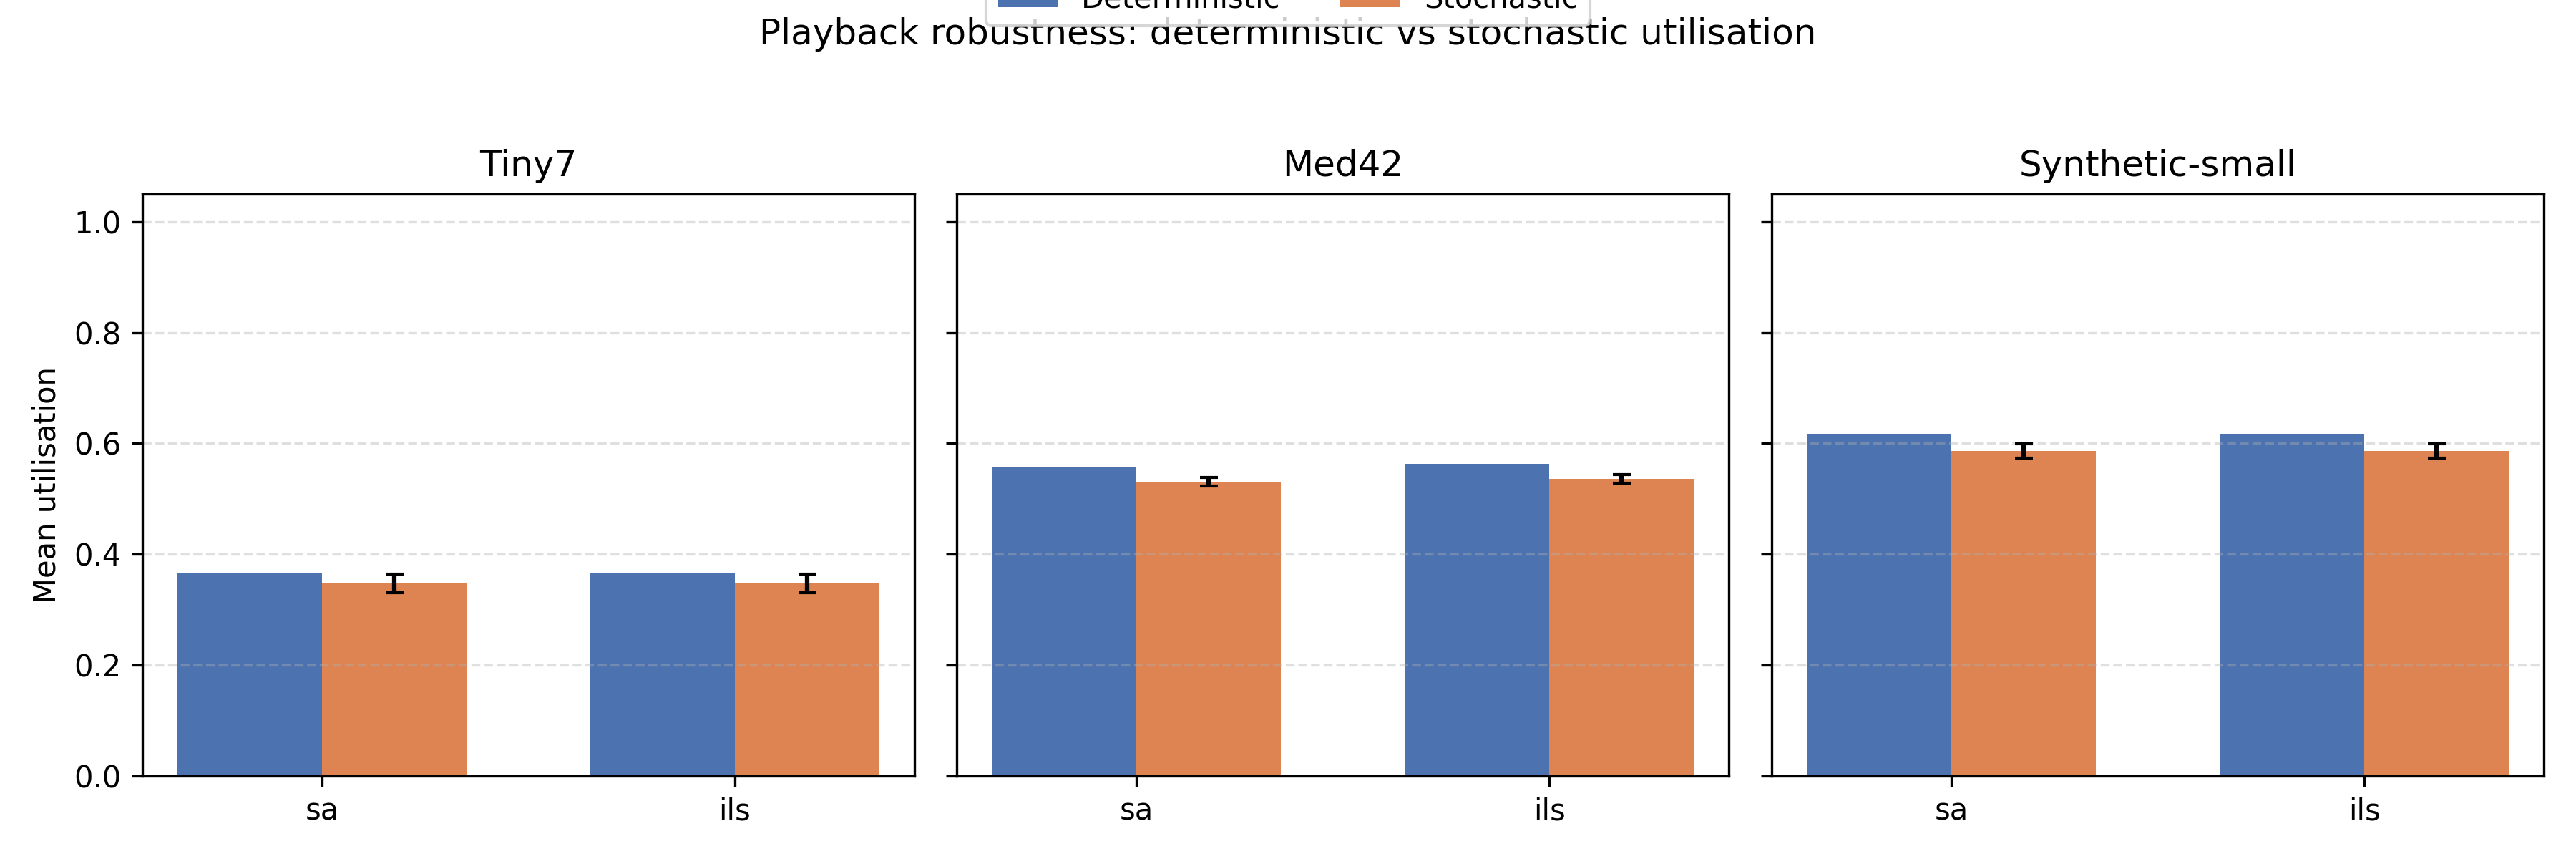
\includegraphics[width=\linewidth]{sections/includes/utilisation_robustness.png}
  \caption{Deterministic vs. stochastic utilization across scenarios. Points denote mean day-level utilization and error bars denote standard deviation over stochastic samples.}
  \label{fig:playback}
\end{figure}

\subsection{Operational question 3: cost interpretation and scaling behavior}
Cost summaries complement utilization and production metrics by translating schedule effects into operating implications. On med42, mobilisation cost in Table~\ref{tab:benchmarks} spans 9846.12--10662.28~CAD across solver choices, indicating that comparable schedule quality can imply different movement-cost profiles. In this baseline, costing is used for within-study comparison, not external economic extrapolation.

Scaling results from synthetic tiers (Figure~\ref{fig:scaling}) show increasing runtime under fixed solver budgets: 31.81~s (small, 4 blocks), 84.88~s (medium, 8 blocks), and 108.97~s (large, 16 blocks). The value is a reproducible scale signal measured in the same platform used for benchmark and robustness reporting.

\begin{figure}[t]
  \centering
  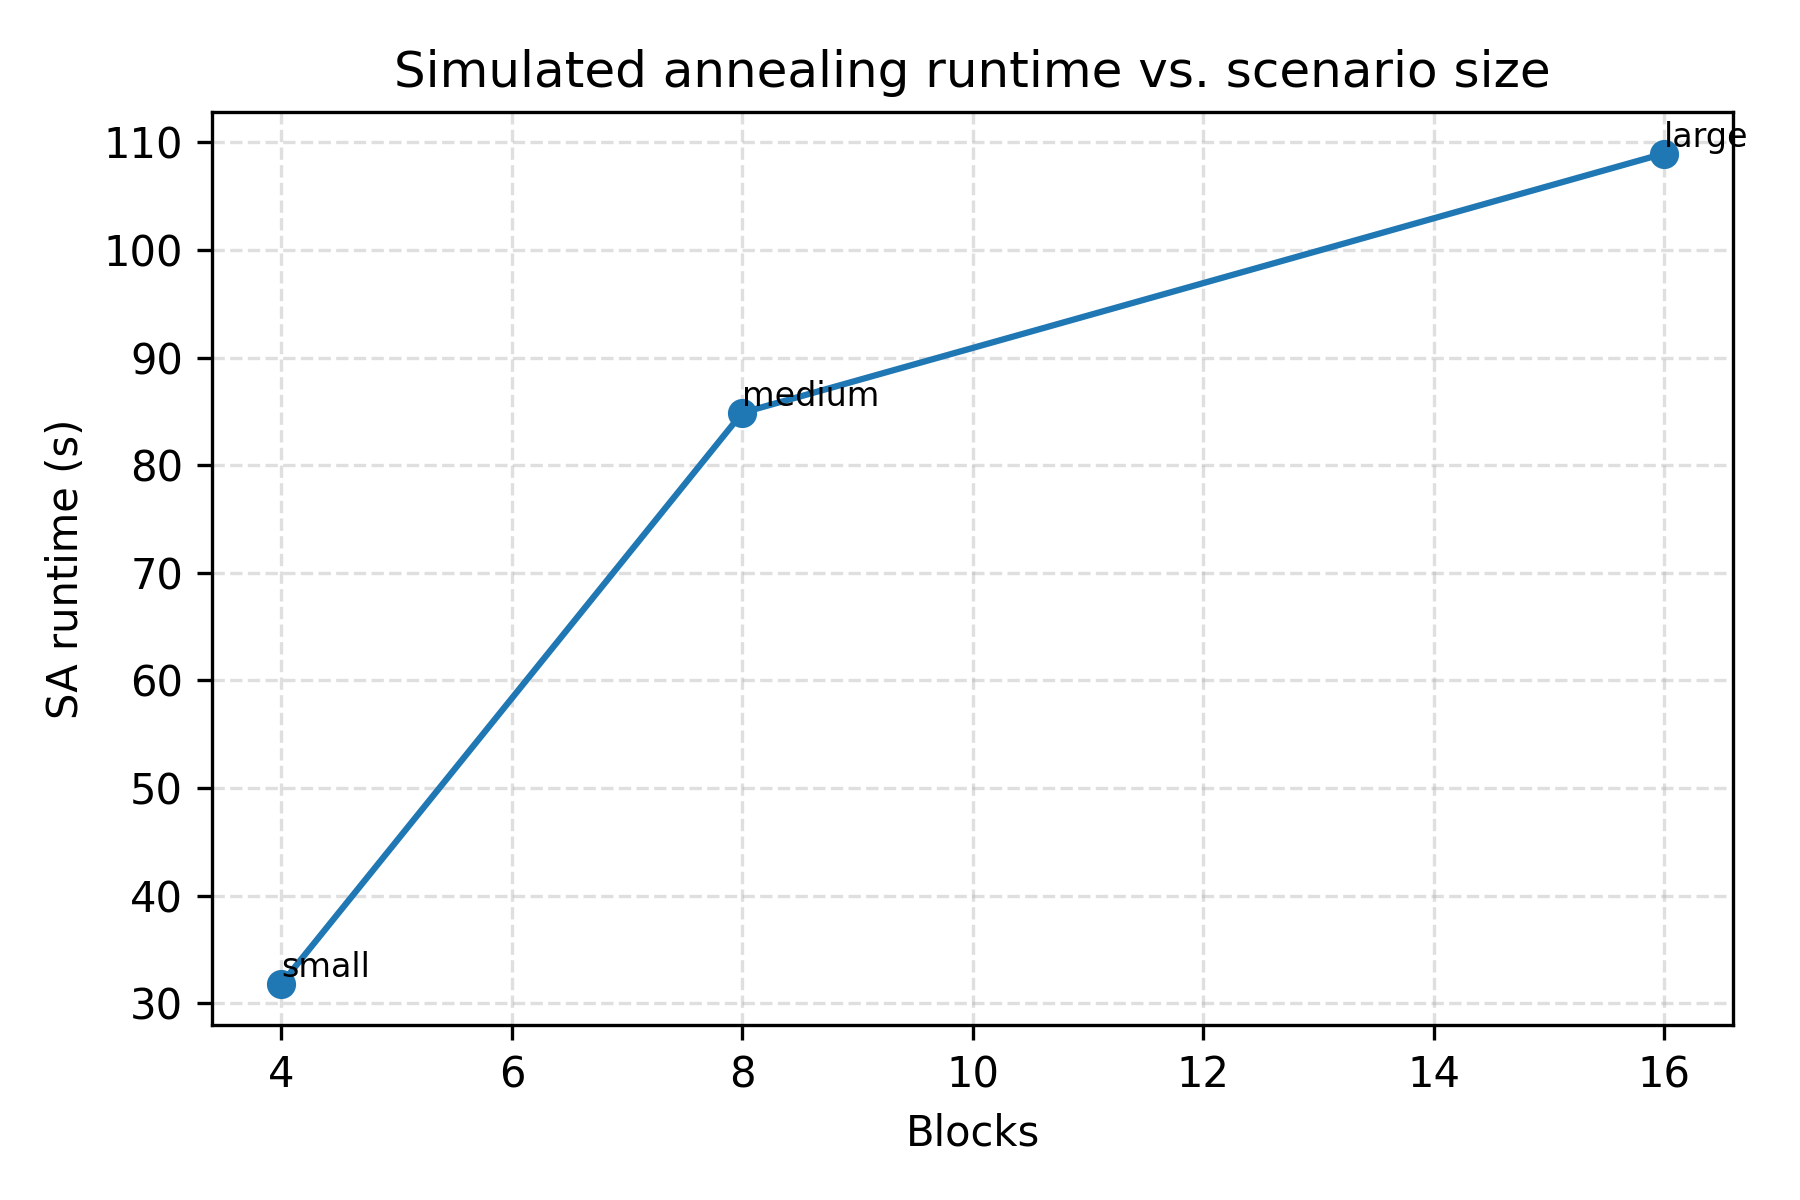
\includegraphics[width=0.8\linewidth]{sections/includes/runtime_vs_blocks.png}
  \caption{Simulated annealing runtime versus number of blocks for synthetic tiers (small, medium, large).}
  \label{fig:scaling}
\end{figure}

\subsection{Scope boundaries and interpretation limits}
Three limits are essential for correct use of this section:
\begin{itemize}
  \item The public ladder currently represents one BC ground-based archetype; broader system families remain out of scope here.
  \item Objective values are comparable within scenario only; cross-scenario interpretation should rely on secondary KPIs (e.g., production, utilization, cost) and relative trends.
  \item Absolute runtime depends on hardware and solver budgets; comparisons in this manuscript are most reliable as within-study baselines.
\end{itemize}

\subsection{Provenance notes}
All tables and figures in this section are generated from versioned manuscript assets and linked run logs so readers can audit values and reuse the same baseline in companion modelling analyses.

% Section 4: Impact
\section{Impact}
\label{sec:impact}

\subsection{Practical value for operations planning}
FHOPS reduces the cost of moving from ad hoc local models to comparable, auditable planning studies. The practical value is not one ``best'' solver run, but a repeatable workflow that keeps inputs, constraints, solver settings, and evaluation outputs aligned across planning cycles.
For planning teams, this supports more defensible schedule revisions because performance differences can be tied to declared assumptions rather than undocumented preprocessing or solver-configuration changes.

\subsection{Research value in the manuscript sequence}
Relative to the review paper \cite{jaffray2025systematic}, this manuscript contributes executable infrastructure: a shared scenario contract, a traceable formulation, and reproducible baseline evidence. Relative to companion modelling studies, it provides the stable software and data baseline used to test methodological questions (e.g., rolling-horizon configuration effects), so platform and modelling claims can be evaluated separately.

\subsection{Maturity and current scope}
The current release is an early public platform baseline. It demonstrates reproducible scheduling experiments on public BC reference scenarios and synthetic tiers (Section~\ref{sec:illustrative-example}), but does not claim broad external deployment evidence.

\subsection{Transferability and limits}
FHOPS is structured to support transfer to new contexts through scenario and parameter updates rather than solver rewrites. Three current limits remain explicit:
\begin{itemize}
  \item Validation breadth is still centered on the current public reference ladder.
  \item Runtime comparisons are environment-dependent and should be interpreted as within-study baselines.
  \item Warm-start MIP integration is implemented, but decisive performance gains at larger stress cases are not yet claimed.
\end{itemize}

These limits keep the manuscript's claims aligned with demonstrated evidence.

% Section 5: Conclusions and future work
\section{Conclusions}
\label{sec:conclusions}

This paper contributes a reusable forest operations scheduling platform positioned between review and companion modelling analyses.

We make three claims supported by evidence in Sections~\ref{sec:software-description} and \ref{sec:illustrative-example}:
\begin{enumerate}
  \item FHOPS provides a domain-aligned planning structure (scenario contract, solver pathways, and evaluation outputs) that supports repeatable operational scheduling studies.
  \item The operational MILP is documented in canonical form with equation-to-code traceability, allowing direct technical audit from manuscript equations to implementation and tests.
  \item Benchmark, robustness, costing, and scaling outputs are reproducibly generated and reusable as a common experimental baseline.
\end{enumerate}

We state three limits explicitly:
\begin{enumerate}
  \item Validation breadth is currently limited to the public BC ground-based reference ladder and synthetic scaling tiers.
  \item Runtime values are hardware- and budget-dependent and should be interpreted primarily as within-study comparisons.
  \item Warm-start MIP support is integrated, but larger-instance performance gains are not yet claimed as established results.
\end{enumerate}

Immediate next work is to use this platform baseline for rolling-horizon and broader deployment studies while preserving the same scenario contract and traceability standards.

% Acknowledgments / declarations
\section*{Acknowledgments}

The authors acknowledge the Forest Resources and Ecosystem Services Hub (FRESH) at the
University of British Columbia for the research environment in which FHOPS was developed.

\section*{Funding}

This research did not receive any specific grant from funding agencies in the public,
commercial, or not-for-profit sectors.

\section*{Declaration of competing interest}

The authors declare that they have no known competing financial interests or personal
relationships that could have appeared to influence the work reported in this paper.

\section*{CRediT author statement}

Gregory Paradis: Conceptualization, Methodology, Software, Validation, Formal analysis,
Data curation, Writing -- original draft, Writing -- review and editing, Visualization,
Project administration. Rosalia Jaffray: Conceptualization, Methodology, Validation,
Investigation, Writing -- original draft, Writing -- review and editing. Kathleen
Coupland: Conceptualization, Methodology, Writing -- review and editing.

\section*{Data availability}

The FHOPS source code is available from the public GitHub repository and PyPI package
record listed in the software metadata tables. Manuscript build scripts, benchmark
summaries, generated tables, and figures are available from the public
\texttt{fhops-manuscript} repository where redistribution terms allow. Bibliographic
references are cited in the manuscript; downloaded reference documents are not
redistributed publicly when copyright or licence terms do not clearly permit it.

\section*{Declaration of generative AI and AI-assisted technologies}

During manuscript preparation, the authors used OpenAI ChatGPT/Codex and command-line
agent tooling to assist with repository maintenance, build troubleshooting,
documentation edits, and manuscript text revision. The authors reviewed, tested, and
revised the generated output and take full responsibility for the content of this
publication.


\bibliographystyle{elsarticle-num}
\bibliography{references}

\end{document}
